\documentclass[]{article}
\usepackage{lmodern}
\usepackage{amssymb,amsmath}
\usepackage{ifxetex,ifluatex}
\usepackage{fixltx2e} % provides \textsubscript
\ifnum 0\ifxetex 1\fi\ifluatex 1\fi=0 % if pdftex
  \usepackage[T1]{fontenc}
  \usepackage[utf8]{inputenc}
\else % if luatex or xelatex
  \ifxetex
    \usepackage{mathspec}
  \else
    \usepackage{fontspec}
  \fi
  \defaultfontfeatures{Ligatures=TeX,Scale=MatchLowercase}
\fi
% use upquote if available, for straight quotes in verbatim environments
\IfFileExists{upquote.sty}{\usepackage{upquote}}{}
% use microtype if available
\IfFileExists{microtype.sty}{%
\usepackage{microtype}
\UseMicrotypeSet[protrusion]{basicmath} % disable protrusion for tt fonts
}{}
\usepackage[margin=1in]{geometry}
\usepackage{hyperref}
\hypersetup{unicode=true,
            pdftitle={Food Balance Sheet workflow in the Statistical Working System},
            pdfauthor={Cristina Muschitiello Food and Agriculture Organization of the United Nations},
            pdfborder={0 0 0},
            breaklinks=true}
\urlstyle{same}  % don't use monospace font for urls
\usepackage{longtable,booktabs}
\usepackage{graphicx,grffile}
\makeatletter
\def\maxwidth{\ifdim\Gin@nat@width>\linewidth\linewidth\else\Gin@nat@width\fi}
\def\maxheight{\ifdim\Gin@nat@height>\textheight\textheight\else\Gin@nat@height\fi}
\makeatother
% Scale images if necessary, so that they will not overflow the page
% margins by default, and it is still possible to overwrite the defaults
% using explicit options in \includegraphics[width, height, ...]{}
\setkeys{Gin}{width=\maxwidth,height=\maxheight,keepaspectratio}
\IfFileExists{parskip.sty}{%
\usepackage{parskip}
}{% else
\setlength{\parindent}{0pt}
\setlength{\parskip}{6pt plus 2pt minus 1pt}
}
\setlength{\emergencystretch}{3em}  % prevent overfull lines
\providecommand{\tightlist}{%
  \setlength{\itemsep}{0pt}\setlength{\parskip}{0pt}}
\setcounter{secnumdepth}{5}
% Redefines (sub)paragraphs to behave more like sections
\ifx\paragraph\undefined\else
\let\oldparagraph\paragraph
\renewcommand{\paragraph}[1]{\oldparagraph{#1}\mbox{}}
\fi
\ifx\subparagraph\undefined\else
\let\oldsubparagraph\subparagraph
\renewcommand{\subparagraph}[1]{\oldsubparagraph{#1}\mbox{}}
\fi

%%% Use protect on footnotes to avoid problems with footnotes in titles
\let\rmarkdownfootnote\footnote%
\def\footnote{\protect\rmarkdownfootnote}

%%% Change title format to be more compact
\usepackage{titling}

% Create subtitle command for use in maketitle
\newcommand{\subtitle}[1]{
  \posttitle{
    \begin{center}\large#1\end{center}
    }
}

\setlength{\droptitle}{-2em}
  \title{Food Balance Sheet workflow\\
in the Statistical Working System}
  \pretitle{\vspace{\droptitle}\centering\huge}
  \posttitle{\par}
  \author{Cristina Muschitiello\\
Food and Agriculture Organization of the United Nations}
  \preauthor{\centering\large\emph}
  \postauthor{\par}
  \predate{\centering\large\emph}
  \postdate{\par}
  \date{25 May 2018}

\usepackage{lscape}
\usepackage{booktabs}
\usepackage{longtable}
\usepackage{array}
\usepackage{multirow}
\usepackage[table]{xcolor}
\usepackage{wrapfig}
\usepackage{float}
\usepackage{colortbl}
\usepackage{pdflscape}
\usepackage{tabu}
\usepackage{threeparttable}
\usepackage{threeparttablex}
\usepackage[normalem]{ulem}
\usepackage{makecell}

\usepackage{draftwatermark}
\usepackage{makeidx}
\makeindex
\usepackage{float}
\floatplacement{figure}{H}
\usepackage{amsmath}
\usepackage{amssymb}
\usepackage{amsthm}
\usepackage{mathtools}

\begin{document}
\maketitle
\begin{abstract}
This vignette provides a description of the workflow and dependencies of
operations in the Statistical Working System for the production of Food
Balance Sheets.
\end{abstract}

{
\setcounter{tocdepth}{4}
\tableofcontents
}
\listoftables

\listoffigures

\newpage

\subsection*{Disclaimer}\label{disclaimer}
\addcontentsline{toc}{subsection}{Disclaimer}

This Working Paper should not be reported as representing the official
view of the FAO. The views expressed in this Working Paper are those of
the author and do not necessarily represent those of the FAO or FAO
policy. Working Papers describe research in progress by the authors and
are published to elicit comments and to further discussion.

This paper is dynamically generated on \today{} and is subject to
changes and updates.

\section*{Variables of The FBS}\label{variables-of-the-fbs}
\addcontentsline{toc}{section}{Variables of The FBS}

The process of creating FBSs starts by collecting all data for the
different variables of the \emph{Food Balance Sheet} equation\footnote{For
  definitions and an extended description of the motivation behind the
  development of FBS, see FAO, 2001, \emph{Food Balance Sheets: A
  Handbook}, available at:
  \url{http://www.fao.org/docrep/003/X9892E/X9892E00.HTM}. Accessed on
  19 January 2017. Moreover see \emph{Standardization \& Balancing for
  Food Balance Sheet Calculation}, in the \emph{Standardization \&
  Balancing} module's documentation on
  \href{https://github.com/SWS-Methodology/faoswsStandardization/tree/master/documentation}{\emph{GitHub}}}:

\begin{equation}
\label{eq:balance1}
P_{ijt} + I_{ijt} - X_{ijt} - \Delta St_{ijt} = FP_{ijt} + Fo_{ijt} + Fe_{ijt} + Lo_{ijt} + Se_{ijt} + IU_{ijt} + T_{ijt}  + ROU_{ijt}
\end{equation}

where the \(i\) index runs over all countries, the \(j\) index over all
commodities, and \(t\) over years and where, dropping indices for
brevity:

\begin{itemize}
\tightlist
\item
  \(P\)=Production
\item
  \(I\)=Imports
\item
  \(X\)=Exports
\item
  \(S\)=Stock level
\item
  \(\Delta St_{t}\) = Stock Variation = \(St_{t} - St_{t-1}\)
\item
  \(FP_{ijt}\) = Food Processing
\item
  \(Fo\)=Food availability
\item
  \(Fe\)=Feed
\item
  \(Lo\)=Losses
\item
  \(Se\)=Seed
\item
  \(IU\)=industrial use
\item
  \(T\)=Tourist consumption
\item
  \(ROU\)=Residual Other Use
\item
  \(TS = Total supply = P_{ijt} + I_{ijt} - \Delta St_{ijt}\)
\end{itemize}

At international level, the primary data source that FAO uses to compile
the the Supply Utilization Accounts/Food Balance Sheets are the data as
collected through the annual \emph{Agriculture Production
Questionnaires}. Unfortunately, measured values are mostly limited to
variables on the supply side (production, imports and exports), while,
on the demand side, most values are imputed data\footnote{For more
  details on FBS variables please see the latest version of the
  \emph{Resource Book}}. The Variables of the FBS are:

\begin{itemize}
\item
  \emph{Production (P)}: Data on production are data at farmgate level.
  As data on production are very important for countries, these data are
  very often survey-based data. Nevertheless, not all countries collect
  data of production for all commodities. Therefore other data
  collection methods are used, like records of private firms and
  commodity organization. When no other data are available, Production
  figures are imputed or estimated. Imputation and estimation procedures
  depends on the specific commodity. There are different procedures for
  crops and livestock but all based on an \emph{ensemble approach}.
  Production data in the FBS framework are collected, imputed or
  estimated for all the primary commodities and for a set of derived
  commodities\footnote{See \emph{Production module} documentation for
    more details on procedures and list of commodities}.
\item
  \emph{Import(I) and Export(X)}: Data on Trade are, mainly, official
  from international trade databases, like UNSD and EUROSTAT, at HS6
  commodity level\footnote{Harmonized Commodity Description and Coding
    Systems (HS) is an internationalclassification of products held by
    UNSD. Is made of six-digit level codes and used worldwide for
    trading data classifications. See official
    \href{https://unstats.un.org/unsd/tradekb/Knowledgebase/50018/Harmonized-Commodity-Description-and-Coding-Systems-HS}{\emph{HS6
    UNSD webpage}} for mode details}. Official data are integrated with
  supplementary data having the main aim of filling in all the
  information hidden by the unrecorded trade and coming, mainly, from
  trading partners. HS6 classification is more detailed than the used
  CPC classiffication, therefore, these data are aggregated in CPC
  commodities before being used in the standardization process\footnote{See
    \href{https://github.com/SWS-Methodology/faoswsTrade/blob/master/vignettes/Documentation/tradeDocumentation.pdf}{\emph{Trade
    module}} documentation for more details}.
\item
  \emph{Stock Variation (}\(\Delta St_{t})\): In the FBS framework,
  stocks are considered as \emph{changes in stocks} from one time period
  to the next. Moreover they are considered as a component of supply.
  Therefore, the \(-\) sign indicates that the stock is decreased, which
  means that the stocks are available as a supply, while the \(+\) sign
  indicates that the stocks have increased and they are, therefore,
  considered as a utilization for that commodity. Changes in stocks are
  tipically limited to a short number of commodities, mainly grains,
  pulses and sugar and, because they are very rarely measured by
  country, figures are very often imputed or estimated\footnote{For a
    complete list of stock commodities and for details about the
    imputation methodology, please refer to specific documentation for
    stock}. Estimation of \emph{changes in stock} is based on opening
  stocks figures throught an approach that mantain time consistency of
  available data and official data\footnote{All data are marked as
    \emph{official}, \emph{semi-official} or \emph{unofficial},
    depending on the source they come from, throught \emph{flags}. Flag
    management is one of the core responsibilities of the \emph{Office
    of the Chief Statistician} Department in FAO. Flags are used from
    all the estimation procedure for distinguishing between different
    level of reliability in the data. The most reliable data are used to
    estimate missing or less reliable data.{[}this has to be better
    specified{]}}.
\item
  \emph{Food availability (Fo)}: Food availability is defined as the
  quantity of any substance that is available for human consumption at
  the retail level by the country's resident population during a given
  reference period. Official data of food availability come from
  questionnaires, industrial ouptut surveys and household consumption or
  expenditure surveys. When these sources of data are not available,
  food availability data are imputated or estimated. Not all CPC
  commodities are Food commodities, as not all commodities are used for
  human consumption. Food commodities are divided in two main groups:
  \emph{Food Estimates} and \emph{Food Residual} and estimated
  differently depending on the pertaining group, respectively as linear
  or logaritmic function of income elasticity of demand, GDP per capita,
  and population, or as residual quantity of production and net trade
  quantities\footnote{For a complete list of food commodities of the two
    typologies and for details about the imputation methodology, please
    refer to specific documentation for Food availablity}.
\item
  \emph{Feed (Fe)}: Feed demand is increasing because of the increase in
  income of developing countries. Animal feed may vary among countries
  due to the difference in livestock and the diversity of commodity used
  for livestock's rations. Official feed demand data might be available
  from specific questionnaires. Even when available, these data need to
  be cross-checked against livestock availability in terms of
  requirements. When official data, and also other sources of
  semi-official data, are not available, feed data are estimated as a
  function of livestock availability and livestock feed demand in terms
  of energy and protein requirements, in accordance with an inventory of
  the potential feed supply's products of any country.
\item
  \emph{Seed (Se)}: Official seed data may come from agricultural
  surveys, while other sources of data might be found in some technical
  publication. When data are not available these are estimated as a
  function of a seeding rate and a sown area in the following year.
\item
  \emph{Tourism Consumption (T)}: Tourism consumption is considered here
  as a separate utilization variable, while in the past it was included
  in the ``other utilization'' catchall cathegory. Official data for
  this variable are rare and may come from tourism offices or collected
  by tourism boards through surveys. UNWTO is an alternative source of
  data, but other authorities might also be used. Imputations and
  estimations of tourist food are made as a function of food figures.
\item
  \emph{Industrial Use (IU)}: This variable refers to utilization of any
  food items in any non-food industry. Non-food use of food commodities
  is growing and is highly context and country specific. For this reason
  there are not, at the moment, suggestions on how to impute and
  estimate missing figures. As a consequence, Industrial data available
  for Food Balance Sheets are only those coming from Official or
  unofficial sources. At the moment the data used comes from USDA and
  from questionnaries.
\item
  \emph{Loss (L)}: FAO has developed the Global Food Loss Index (GFLI)
  that focuses on the supply-side aspects of improving the efficiency of
  global food supply chains. The index is based on a set of primary
  commodities that are key in agricultural production systems, including
  crops, livestock, and fisheries. In order to track losses without
  compounding production variability, losses are expressed as a
  percentage and are aggregated using fixed quantities and prices. The
  primary data source that FAO uses for compiling GFLI are loss factors
  as collected by Questionnaires. Other sources are publications and
  reports from subnational reports, academic institutions, international
  organizations and so on. The missing data are imputed using a
  hyerarchical model based on commodity groups\footnote{ask for links to
    a proper documentation}.
\item
  \emph{Residual and other use (ROU)}: ROU is used to capture categories
  of products that do not follow in any other category and that might be
  considered ``not important'' for the FBS scope. Normally, these
  residual commodities are different from country to country and for
  this reason they fall in this variable. ROU are set not to be higher
  that 5\% of total supply and are calculated at-post as absorbing
  element, in the sense that it absorbs part or all of the imbalance
  that may exist, at FBS commodity aggregate level, after the
  standardization process. Any imbalance bigger than 5\% of total supply
  is balanced thrugh a balancing mechanism that will be later specified.
\item
  \emph{Food Processing (FP)}: This variable represents the amount of
  the availability of a commodity that enters a manufacturing process to
  be transformed into a derived commodity. Food processing is not
  officially measured, nor collected via official sources. This variable
  is entirely calculated during the standardization process by applying
  extraction rates to the amount of production of the derived commodity.
  This will be better specified in section \emph{2-Step2} of the present
  document.
\end{itemize}

The data of each variable are generally checked and imputed in time
series. The set of operations required for creating/checking time series
of data for each variable is called \emph{module}. A
\textbf{\emph{module}}, in the FBS Framework, is an R-script, written by
an R-developer and integrate inside the \textbf{\emph{Statistical
Working System (SWS)}}\footnote{SWS is an internal Working System
  providing a platform for statisticians and statistical clers to
  collect, collate, validate and correct data. Moreover, the platfors
  supports the possibility of performing imputations of data based on
  statisticians' knowledge and development.} by means of \emph{plugins}.
There is at least one module (there might be more) for each variable of
the FBS. Each module produces figures that are collected in a dataset
inside the SWS for future uses or publication. Output data of a module
may become input data of another module, this circumstance creating a
precise sequence for the execution of a complete FBS.

\section*{Definitions}\label{definitions}
\addcontentsline{toc}{section}{Definitions}

there are 8 main thypologies of objects that will be use in the present
document. These correspond to objects that are used in the SWS in
managing processes:

\begin{enumerate}
\def\labelenumi{\arabic{enumi}.}
\tightlist
\item
  \textbf{\emph{Domain}}: A domain is an area of work where other
  objects are grouped, by a common criterion of interest.
\item
  \textbf{\emph{Data}}: In this framework, every information is grouped
  under this name, which will be characterized by its origin, whether it
  is collected or created.
\item
  \textbf{\emph{Datasets}}: A dataset inside the SWS. Each Dataset can
  belong only to one domain. Datasets allow for:

  \begin{itemize}
  \tightlist
  \item
    metadata management,
  \item
    detailed data hystory
  \end{itemize}
\item
  \textbf{\emph{Data Tables}}: Data Tables are less protected object
  that can be easily modified and do not keep history of data.
\item
  \textbf{\emph{Modules}}: a Module is a process, writte, in this
  context, in R, which performs different typologies of processes:

  \begin{itemize}
  \tightlist
  \item
    data manipulation,
  \item
    statistical analysis,
  \item
    other kind of operations on data.
  \end{itemize}
\item
  \textbf{\emph{Plugin}}: a Plugin is a module when it is integrated
  inside the SWS and executable from any user.
\item
  \textbf{\emph{Data Flow}}: any information's flow or transfer.
\end{enumerate}

For the purposes of this document the following notation will be used:

\begin{figure}[H]

{\centering 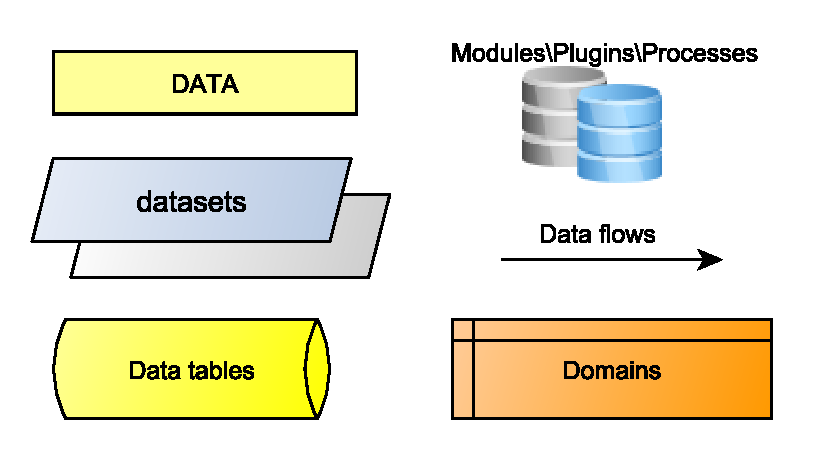
\includegraphics[width=0.7\linewidth]{images/SwsFbs/01_actors} 

}

\caption{\label{fig:f1}Legend of Objects}\label{fig:f1}
\end{figure}

\section*{The actors of the FBS in the
SWS}\label{the-actors-of-the-fbs-in-the-sws}
\addcontentsline{toc}{section}{The actors of the FBS in the SWS}

In the compilation of FBS involves 11 domains:

\begin{enumerate}
\def\labelenumi{\arabic{enumi}.}
\tightlist
\item
  Agriculture production
\item
  Trade
\item
  trade-input-data
\item
  Stock
\item
  Industrial Use
\item
  Food Domain
\item
  Loss and Waste
\item
  Tourism Domain
\item
  SUA/FBS Domain
\item
  United Stated Department of Agriculture
\item
  Population
\item
  faostat\_datasets
\end{enumerate}

Inside these domains 18 datasets and 11 data tables are involved, as
represented in figures Figure \ref{fig:f2} and \ref{fig:f4}. Details on
these objects will be provided along the document.

\section*{The Overall Workflow of the
FBS}\label{the-overall-workflow-of-the-fbs}
\addcontentsline{toc}{section}{The Overall Workflow of the FBS}

The workflow for compiling Food Balance Sheet is articulated and has
dependencies, as some module to run properly might use data that are the
output of other modules.

Figure \ref{fig:f3} presents a simplistic representation of the overall
Worflow. As shown, it consists of 8 propaedeutic steps that will be
described in this document.

\begin{figure}[H]

{\centering 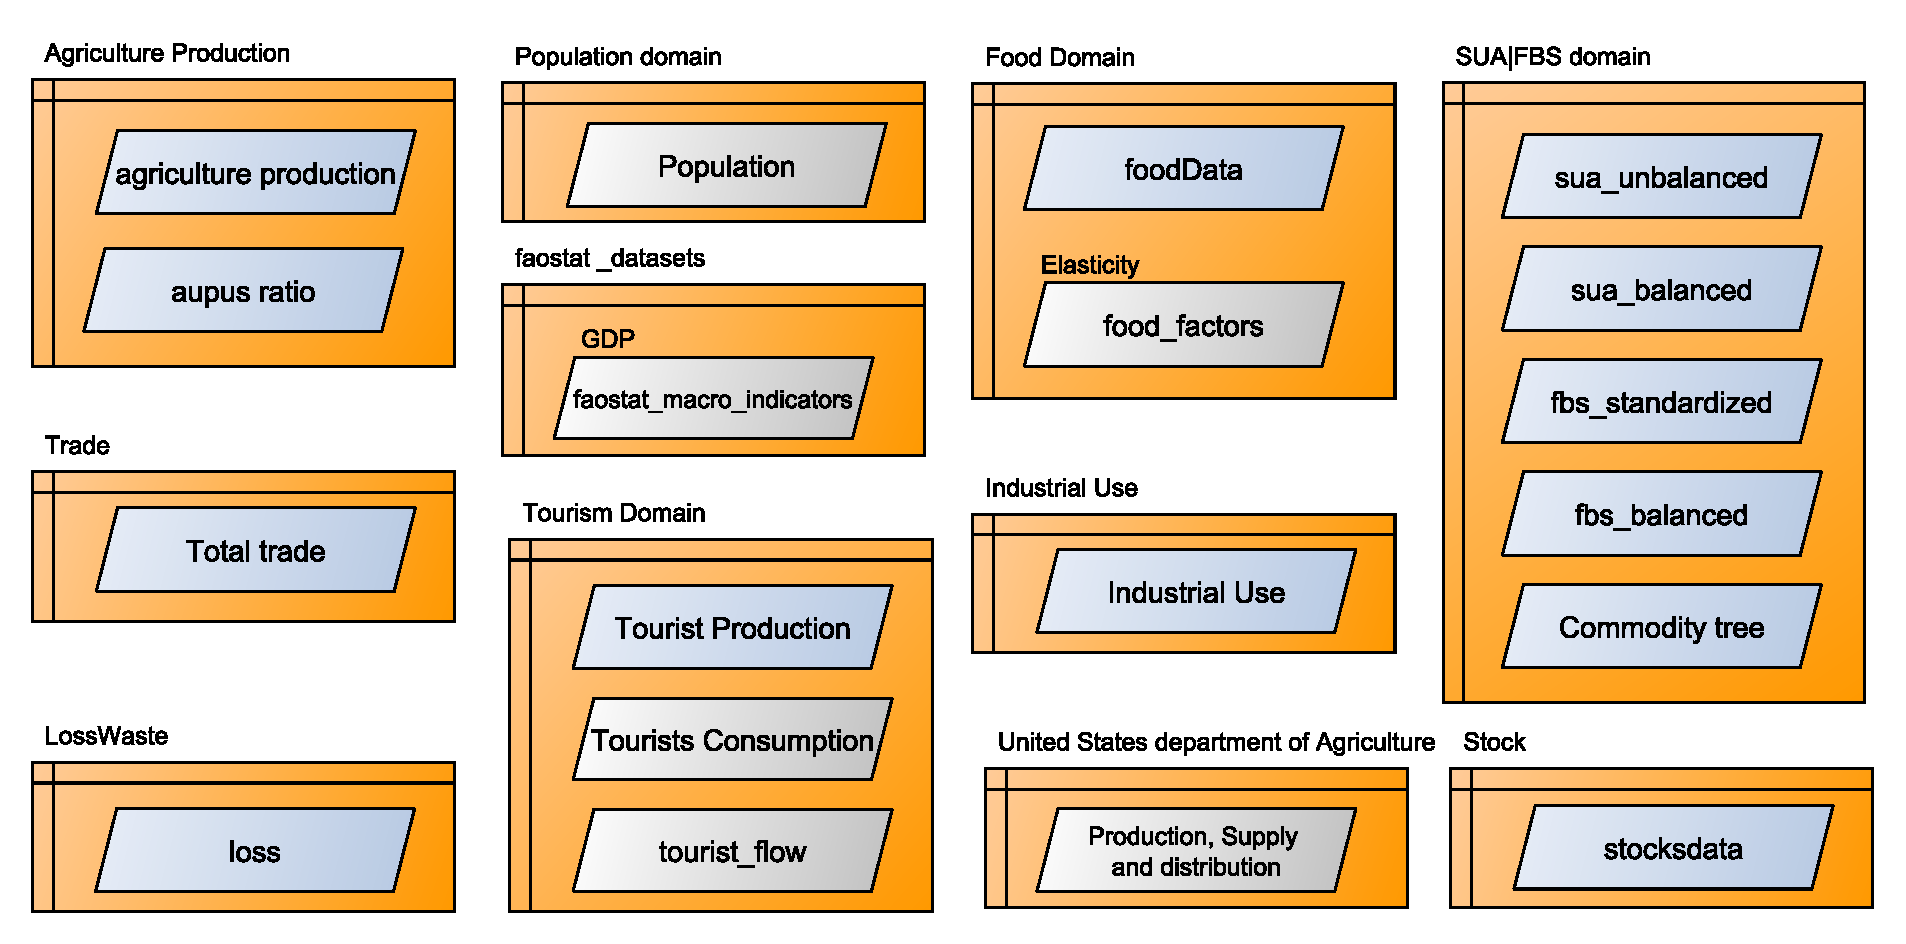
\includegraphics[width=0.9\linewidth]{images/SwsFbs/02_DatasetsDomains} 

}

\caption{\label{fig:f2}FBS Datasets and their domains in the SWS}\label{fig:f2}
\end{figure}

\begin{figure}[H]

{\centering 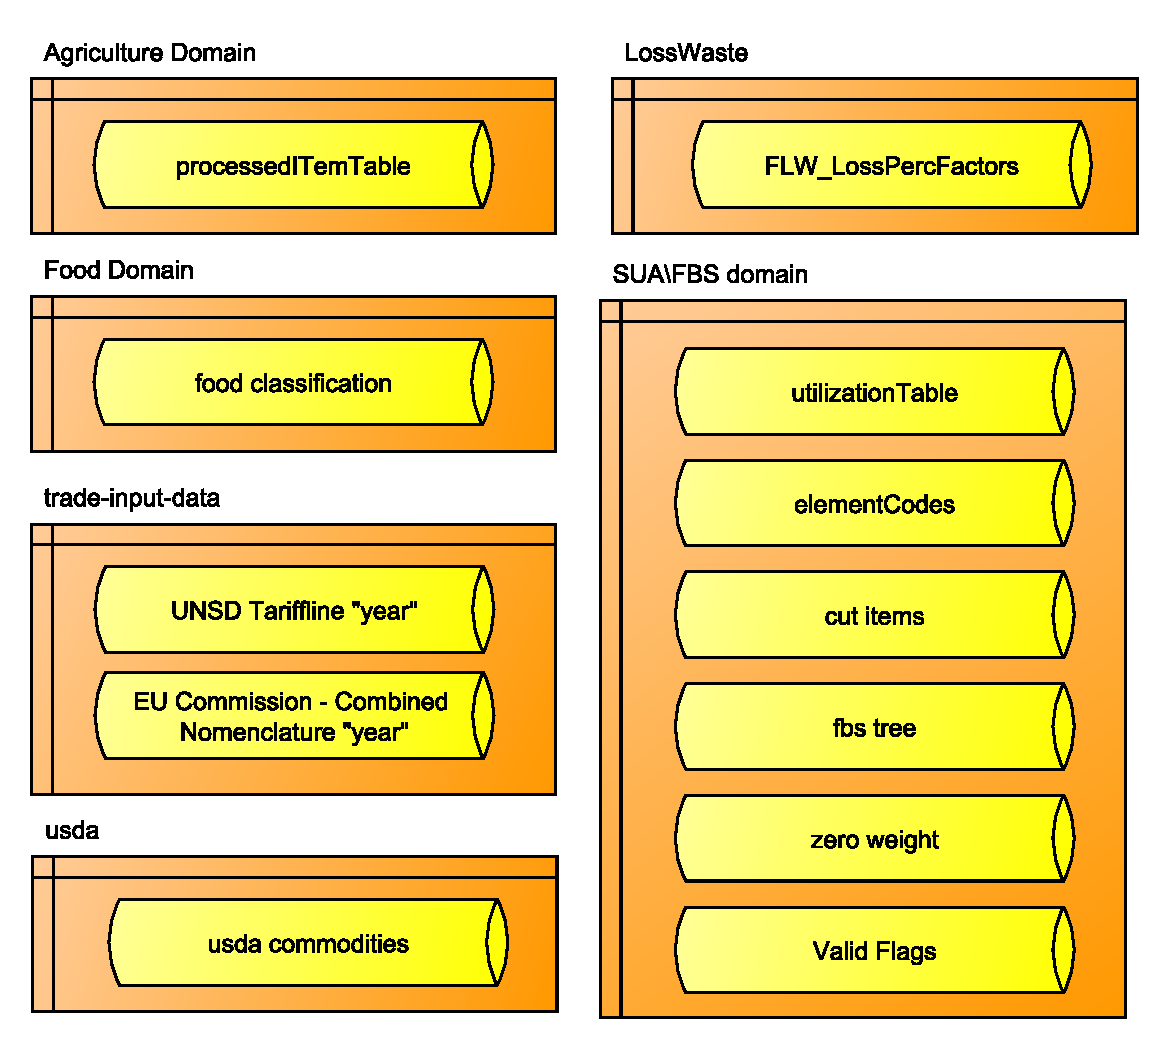
\includegraphics[width=0.9\linewidth]{images/SwsFbs/04_DataTablesDomains} 

}

\caption{\label{fig:f4}FBS Datatables and their domains in the SWS}\label{fig:f4}
\end{figure}

\begin{figure}[H]

{\centering 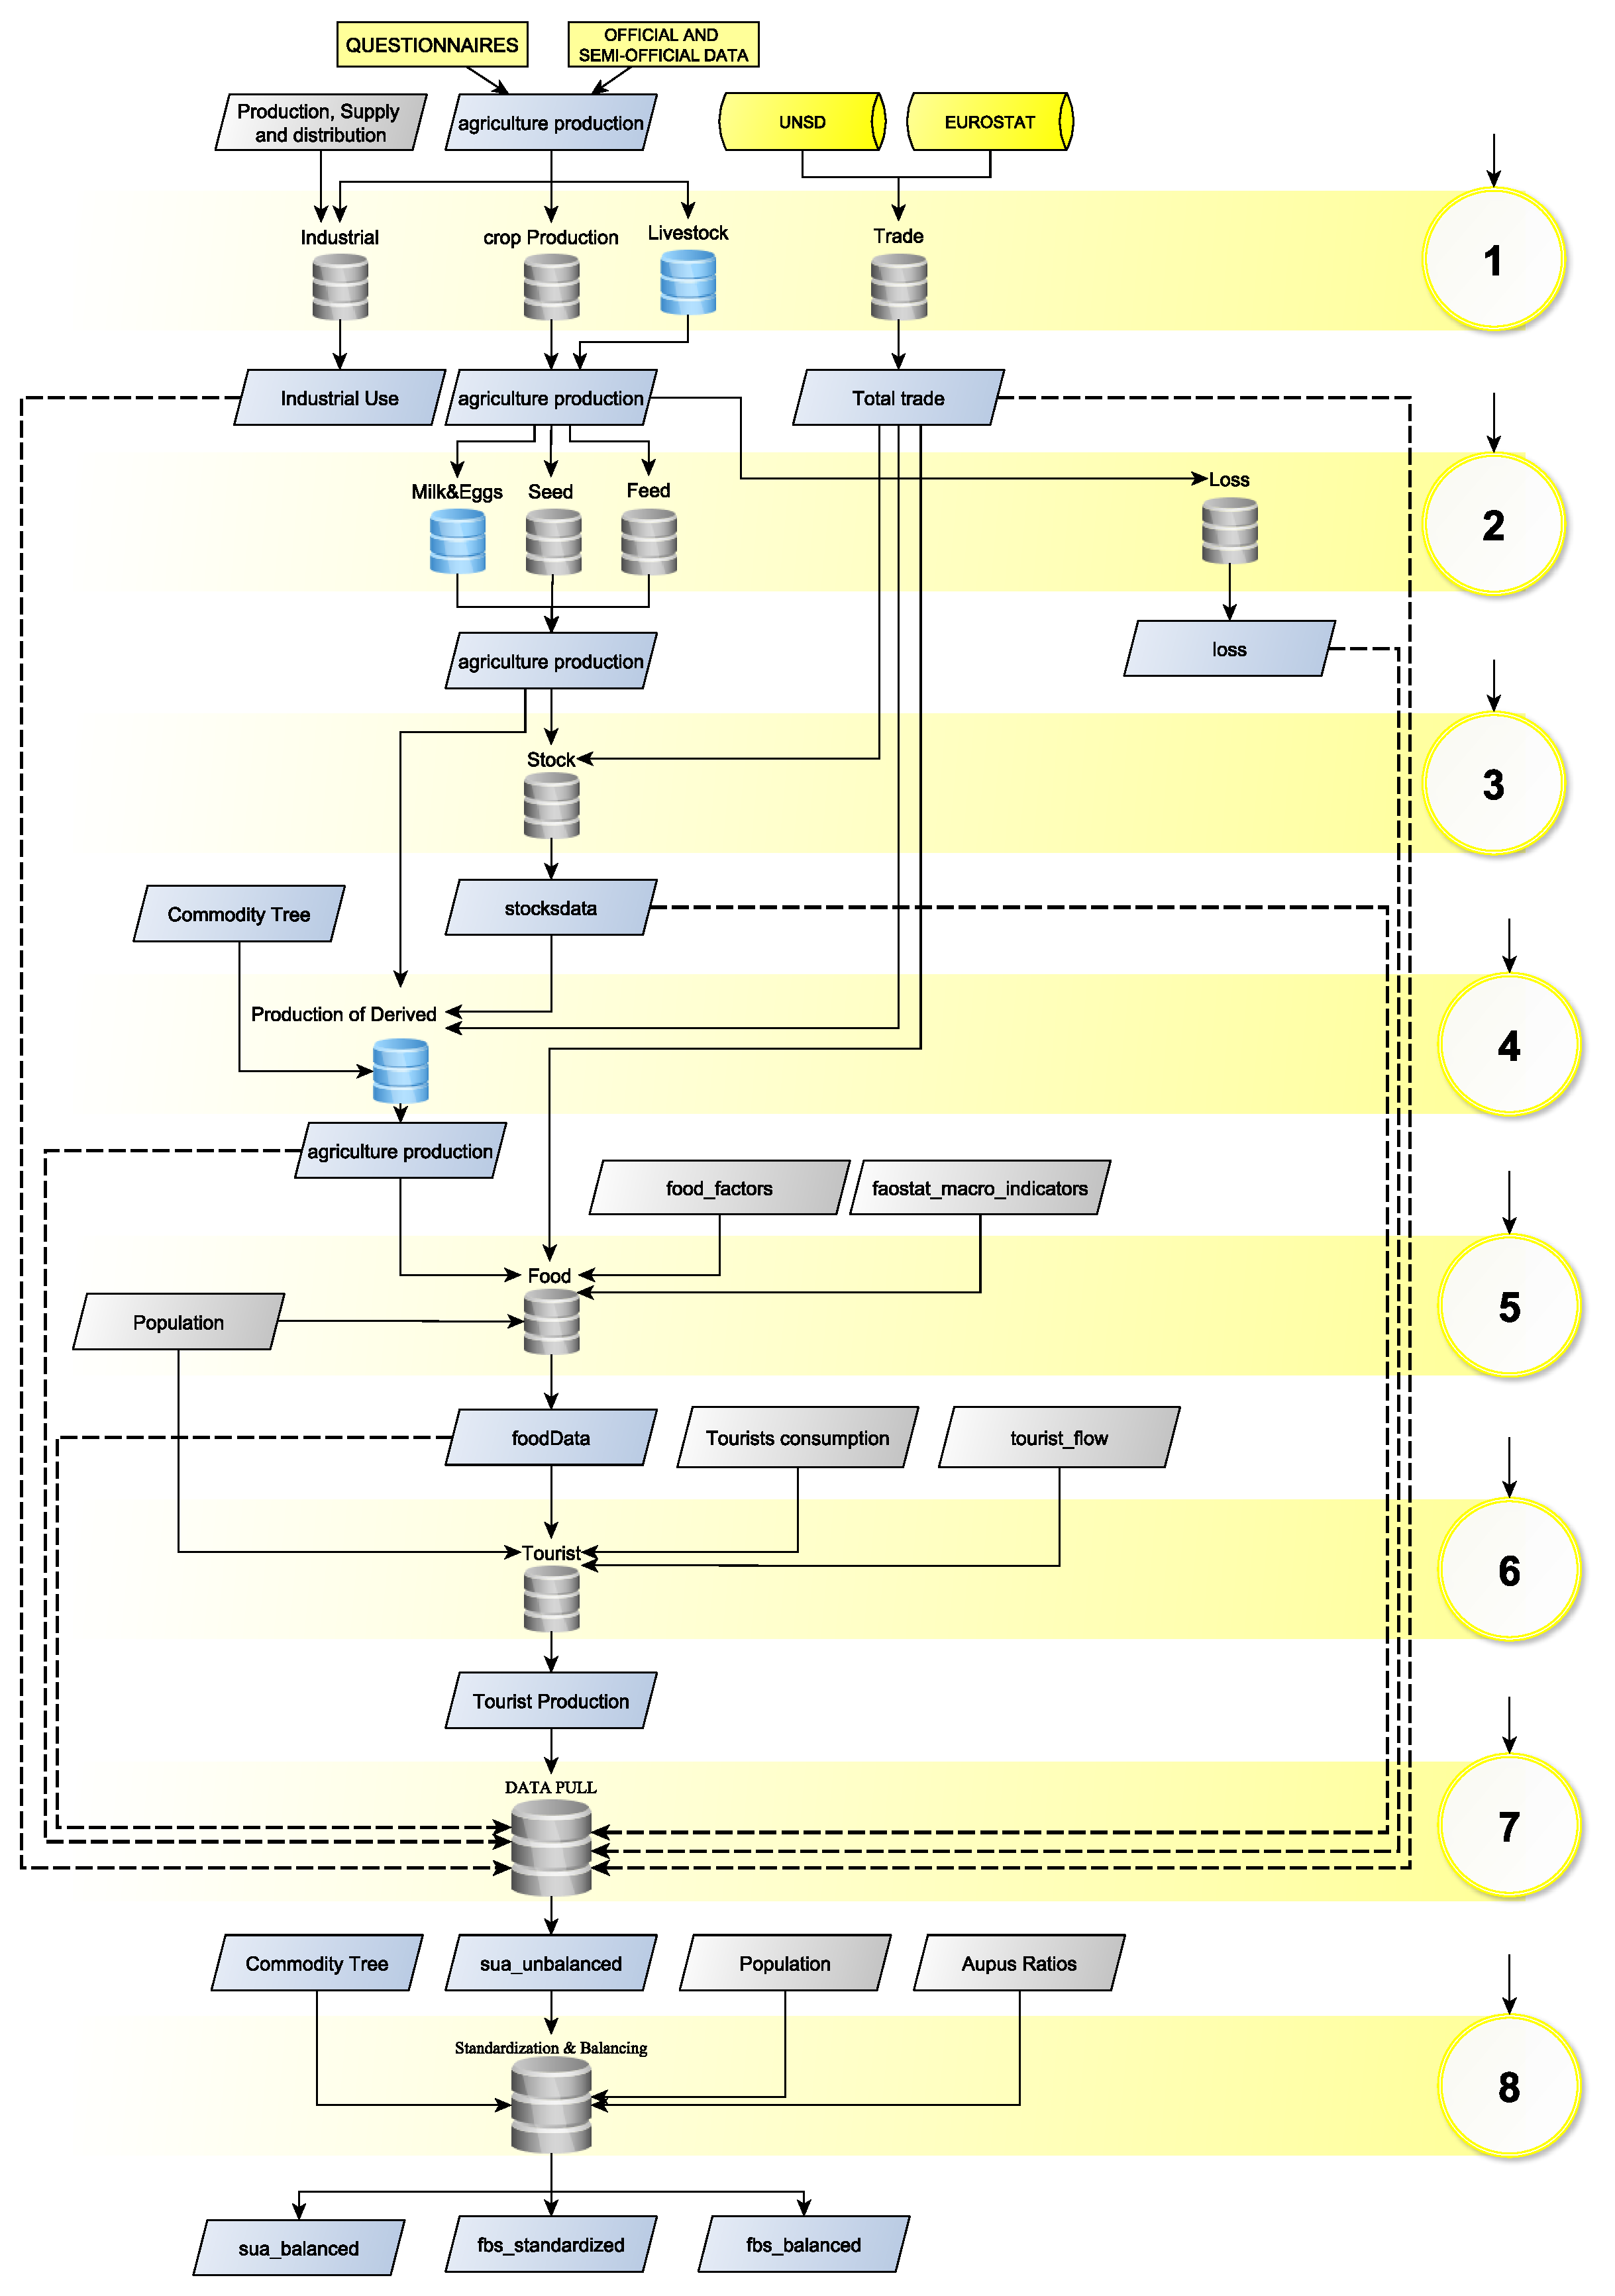
\includegraphics{images/SwsFbs/03_DataFlow_all} 

}

\caption{\label{fig:f3}The overall workflow}\label{fig:f3}
\end{figure}

\section*{Flag Management in the FBS
framework}\label{flag-management-in-the-fbs-framework}
\addcontentsline{toc}{section}{Flag Management in the FBS framework}

Distinction between sources of data in the overall process of poducing
FBS is performed throught Flags. Flags in FAO play a fundamental role
and are managed by the \emph{Office of the Chief Statistician} Division
in FAO\footnote{link some documentation on Flags\ldots{} which one?}. In
the context of FBS flags are used accordingly to a table (stored in teh
SWS as Data table in the SUA/FBS domain) which set the combination of
flags that are assciated to valid, invalid, official, unoffical
estimated data, etc. Table 1 reports the Valid Flag combination in the
SWS, taken from this Data Table.

\begin{longtable}[]{@{}cccc@{}}
\caption{Valid Flag combinations from Valid Flags table}\tabularnewline
\toprule
flagObservationStatus & flagMethod & Valid & Protected\tabularnewline
\midrule
\endfirsthead
\toprule
flagObservationStatus & flagMethod & Valid & Protected\tabularnewline
\midrule
\endhead
E & - & TRUE & FALSE\tabularnewline
E & c & TRUE & TRUE\tabularnewline
E & f & TRUE & TRUE\tabularnewline
E & h & TRUE & TRUE\tabularnewline
E & i & TRUE & FALSE\tabularnewline
E & s & TRUE & FALSE\tabularnewline
I & - & TRUE & FALSE\tabularnewline
I & b & TRUE & FALSE\tabularnewline
I & c & TRUE & TRUE\tabularnewline
I & e & TRUE & FALSE\tabularnewline
I & i & TRUE & FALSE\tabularnewline
I & s & TRUE & FALSE\tabularnewline
M & - & TRUE & FALSE\tabularnewline
M & c & TRUE & FALSE\tabularnewline
M & i & TRUE & FALSE\tabularnewline
M & q & TRUE & FALSE\tabularnewline
M & s & TRUE & FALSE\tabularnewline
M & u & TRUE & FALSE\tabularnewline
T & - & TRUE & TRUE\tabularnewline
T & c & TRUE & TRUE\tabularnewline
T & h & TRUE & TRUE\tabularnewline
T & i & TRUE & FALSE\tabularnewline
T & p & TRUE & TRUE\tabularnewline
T & s & TRUE & FALSE\tabularnewline
& - & TRUE & TRUE\tabularnewline
& c & TRUE & TRUE\tabularnewline
& h & TRUE & TRUE\tabularnewline
& i & TRUE & FALSE\tabularnewline
& p & TRUE & TRUE\tabularnewline
& q & TRUE & TRUE\tabularnewline
& s & TRUE & FALSE\tabularnewline
\bottomrule
\end{longtable}

A specific agreement exists in this context for which all data coming
from old methodology, which are often used for consistency and coherence
with the past, are assigned a \emph{method flag} equal to \emph{``-''}.

\section{Initial data and the first set of modules
run}\label{initial-data-and-the-first-set-of-modules-run}

\subsection{\texorpdfstring{The \emph{Agriculture-aproduction}
dataset}{The Agriculture-aproduction dataset}}\label{the-agriculture-aproduction-dataset}

The data collected throught the \emph{Agriculture Production
Questionnaires} and from other official or semi-official sources are
collected inside the \emph{Agriculture:aproduction} (i.e.
\emph{agriculture domain}, \emph{aproduction} dataset) dataset. Here all
data are collected from countries on:

\begin{itemize}
\tightlist
\item
  Area harvested
\item
  Yield
\item
  Area sawn
\item
  Carcass weight
\item
  Livestock
\item
  Milking animals
\item
  Milking products
\item
  Seed qt
\item
  Crop Production qt
\item
  stocks qt
\item
  Industrial Use qt
\item
  Feed qt
\item
  Food availability qt
\item
  Losses qt
\end{itemize}

It represents the main input dataset containing input-data of almost all
domains (Trade is excluded as it takes data from different sources). It
has a special role in the all FBS framework and its content and use is
very delicate and not straightforward. In particular this dataset
contains different typologies of data, some used as they are and other
used for prosucing other data:

\begin{enumerate}
\def\labelenumi{\arabic{enumi}.}
\tightlist
\item
  Data on area harvested, yield, area sawn are used for estimating
  missing production data and seed data;
\item
  Data on Crop Production, Industrial Use, Feed, Seed, Food and Losses
  originally collected in this dataset are \emph{Protected}, which means
  that they will be used for:

  \begin{itemize}
  \tightlist
  \item
    estimating missing production data,
  \item
    estimating missing seed data,
  \item
    estimating missin feed data,
  \item
    directly used for the FBS calculation
  \end{itemize}
\item
  Data on Carcass weight, livestock, milking animals and milking
  products are used by other modules for producing data on meat, milk
  and eggs.
\end{enumerate}

Indeed, three modules are run which have this dataset, as it is at the
beginning of the overall process, as, unique or not, inpu:

\begin{enumerate}
\def\labelenumi{\arabic{enumi}.}
\tightlist
\item
  Industrial use Module
\item
  crop Production Module
\item
  Livestock Module
\end{enumerate}

\subsubsection{\texorpdfstring{\emph{Industrial use
Module}}{Industrial use Module}}\label{industrial-use-module}

\subsubsection{\texorpdfstring{\emph{crop Production
Module}}{crop Production Module}}\label{crop-production-module}

\subsubsection{\texorpdfstring{\emph{Livestock
Module}}{Livestock Module}}\label{livestock-module}

\subsection{\texorpdfstring{\emph{Trade
Module}}{Trade Module}}\label{trade-module}

\subsubsection{Module on Crop
production}\label{module-on-crop-production}


\end{document}
